
\chapter{Software Structure and Robustness}

The mathematical and numerical robustness of a deterministic computer model depends upon
three issues: the code must be transparent so that it can be understood and modified by visual
inspection; it must be possible to check and verify with automated tools; and there must be a
method for checking the correctness of the solution, at least for asymptotic (steady state)
solutions (numerical stability and agreement with known solutions).
In order to understand the meaning of accuracy and robustness, it is necessary to understand the
means by which the numerical routines are structured. In this chapter, details of the
implementation of the model are presented, including the tests used to assess the numerical
aspects of the model. These include:

\begin{itemize}
\item the structure of the model, including the major routines implementing the various
physical phenomena included in the model,
\item the organization of data initialization and data input used by the model,
\item the structure of data used to formulate the differential equations solved by the model,
\item a summary of the main control routines in the model that are used to control all input and
output, initialize the model and solve the appropriate differential equation set for the
problem to be solved,
\item the means by which the computer code is checked for consistency and correctness,
\item analysis of the numerical implementation for stability and error propagation, and
\item comparison of the results of the system model with simple analytical or numerical
solutions.
\end{itemize}

\section{Structure of the Numerical Routines}

A methodology which is critical to verification of the model is the schema used to incorporate
physical phenomena. This is the subroutine structure discussed below. The method for
incorporating new phenomena and ensuring the correctness of the code was adopted as part of
the consolidation of CCFM and FAST. This consolidation occurred in 1990 and has resulted in a
more transparent, transportable and verifiable numerical model. This transparency is crucial to a
verifiable and robust numerical implementation of the predictive model as discussed in the
sections on code checking and numerical analysis.

The model can be split into distinct parts. There are routines for reading data, calculating results
and reporting the results to a file or printer. The major routines for performing these functions
are identified in figure \ref{figCFASTStructure}. These physical interface routines link the CFAST model to the actual routines which calculate quantities such as mass or energy flow at one particular point in time for a given environment.

\begin{figure}[\figoptions{b}]
\begin{center}
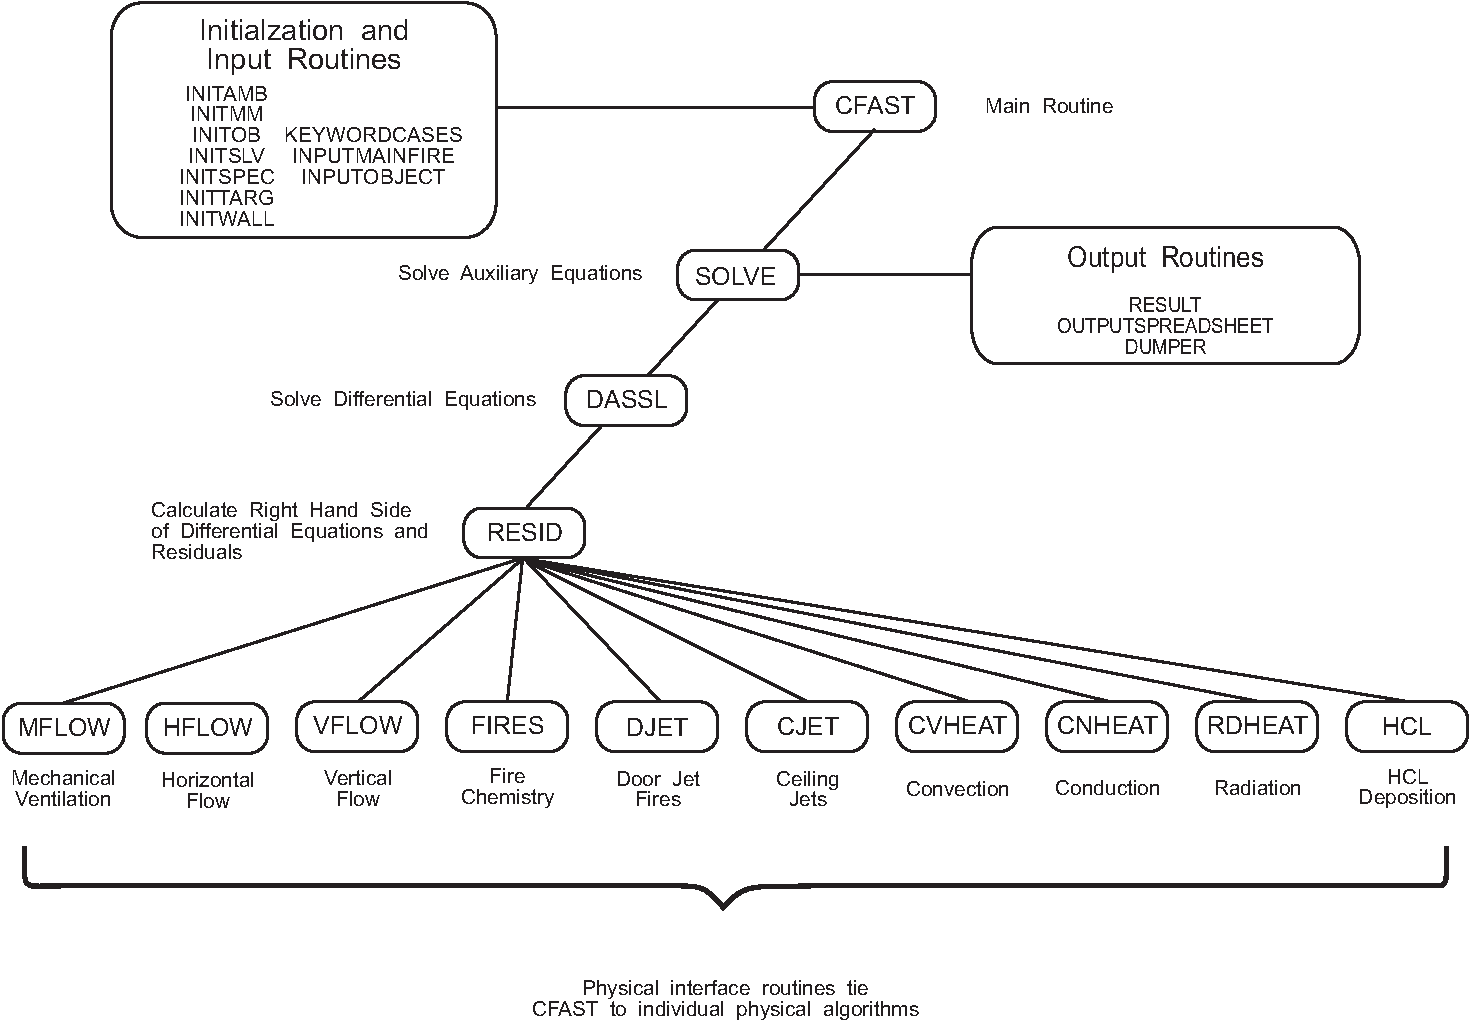
\includegraphics[width=4.4444in]{FIGURES/struct.pdf}\\
\end{center}
\caption[Subroutine structure for the CFAST model]{Subroutine structure for the CFAST model showing major routines and calling structure.}
 \label{figCFASTStructure}
\end{figure}

The routines SOLVE, RESID and DASSL are the key to understanding how the physical
equations are solved. SOLVE is the control program that oversees the general solution of the
problem. It invokes the differential equation solver DASSL \cite{DASSL} which in turn calls RESID to
solve the transport equations. Given a solution at time t, what is the solution at time t plus a
small increment of time, $\dt$? The differential equations are of the form

\begin{eqnarray}
   \frac{{dy}}{{dx}} &=& f(y,t) \label{eqdiffeqform}  \\
    y(t_0 ) &=& y_0 \nonumber
\end{eqnarray}

where $y$ is a vector representing pressure, layer height, mass and such, and $f$ is a vector function that represents changes in these values with respect to time. The term $y_0$ is an initial condition at
the initial time $t_0$. The time increment is determined dynamically by the
program to ensure convergence of the solution at t + $\dt$. The subroutine RESID computes the right hand side of eq \ref{eqdiffeqform} and returns a set of residuals of that calculation to be compared to the values expected by DASSL. DASSL
then checks for convergence. Once DASSL reaches an error limit (defined as convergence of
the equations) for the solution at $t+\dt$, SOLVE then advances the solution of species concentration,
wall temperature profiles, and mechanical ventilation for the same time interval.
Note that there are several distinct time scales that are involved in the solution of this type of
problem. The fastest will be chemical kinetics. This scale by assuming that the
chemistry is infinitely fast. The next larger time scale is that associated with the flow field.
These are the equations which are cast into the form of ordinary differential equations. Then
there is the time scale for mechanical ventilation, and finally, heat conduction through objects.
Chemical kinetic times are typically on the order of milliseconds. The transport time scale are
on the order of 0.1 s. The mechanical ventilation and conduction time scales are typically
several seconds, or even longer. The time step is dynamically adjusted to a value appropriate for
the solution of the currently defined equation set. In addition to allowing a more correct solution
to the pressure equation, very large time steps are possible if the problem being solved
approaches steady-state.

\section{Comparison with Analytic Solutions}

Certain CFAST sub-models address phenomena that have analytical solutions, for example, one dimensional heat conduction through a solid or pressure increase in a sealed or slightly leaky compartment as a result of a fire or fan.  The developers of CFAST use analytical solutions to test sub-models to verify the correctness of the coding of the model as part of the development.  Such verification efforts are relatively simple and the results may not always be published or included in the documentation.  Two additional types of verification are possible.  The first type, discussed in Section 3, �Theoretical Basis,� involves validating individual algorithms against experimental work.  The second involves simple experiments, especially for conduction and radiation, for which the results are asymptotic (e.g., a simple single-compartment test case with no fire, all temperatures should equilibrate asymptotically to a single value).  Such comparisons are common and not usually published.

\section{Code Checking}
Two standard programs have been used to check the CFAST model structure and language.  Specifically, FLINT and LINT have been applied to the entire model to verify the correctness of the interface, undefined or incorrectly defined (or used) variables and constants, and completeness of loops and threads.

The CFAST code has also been checked by compiling and running the model on a variety of computer platforms.  Because FORTRAN and C are implemented differently for various computers, this represents both a numerical check as well as a syntactic check.  CFAST has been compiled for Sun (Solaris), SGI (Irix), Microsoft Windows-based PCs (Lahey, Digital, and Intel FORTRAN), and Concurrent computer platforms.  Within the precision afforded by the various hardware implementations, the model outputs are identical on the different platforms. \footnote{Typically an error limit of one part in $10^6$ which is the limit set for the differential equation solver in the solution of the CFAST equations}

The CFAST Technical Reference Guide \cite{CFAST_Tech_Guide_6} contains a detailed description of the CFAST subroutine structure and interactions between the subroutines.

\section{Numerical Tests}

CFAST is designed to use 64-bit precision for real number calculations to minimize the effects of numerical error.

The differential and algebraic equation solver (called DASSL) has been tested for a variety of differential equations and is widely used and accepted \cite{DASSL}.  The radiation and conduction routines have also been tested against known solutions for asymptotic results \cite{Forney_radiation}.

Coupling between the physical algorithms of the model and the differential equation solver also works to ensure numerical accuracy by dynamically adjusting the time step used by the model to advance the solutions of the equation set. Solution tolerances are set to require solution of the model equations within one part in $10{^6}$. This ensures that the error attributable to numerical solution is far less than that associated with the model assumptions.

